\documentclass[11pt,a4paper]{article}
\usepackage[utf8]{inputenc}
\usepackage[T1]{fontenc}
\IfFileExists{lmodern.sty}{\usepackage{lmodern}}{}
\IfFileExists{french.ldf}{\usepackage[french]{babel}}{\usepackage[english]{babel}}
\usepackage{amsmath,amssymb,amsfonts,amsthm}
\usepackage{geometry}
\geometry{top=2.2cm, bottom=2.2cm, left=2.2cm, right=2.2cm}
\usepackage{booktabs,array,multirow}
\usepackage{enumitem}
\usepackage{xcolor}
\usepackage{tcolorbox}
\tcbuselibrary{skins,breakable}
\usepackage{tikz}
\usetikzlibrary{arrows.meta,positioning,shapes.geometric,calc}
\usepackage[colorlinks=true,linkcolor=blue!60!black,citecolor=teal!70!black,urlcolor=blue!70!black]{hyperref}
\usepackage{fancyhdr}

% Définition des boîtes thématiques (conforme aux normes Master RO Bouira)
\newtcolorbox{propbox}[1]{colback=blue!4!white,colframe=blue!75!black,fonttitle=\bfseries,title={#1},breakable,boxrule=0.8pt}
\newtcolorbox{rembox}[1]{colback=orange!4!white,colframe=orange!80!black,fonttitle=\bfseries,title={#1},breakable,boxrule=0.8pt}
\newtcolorbox{verifbox}{colback=green!4!white,colframe=green!45!black,fonttitle=\bfseries,title=Validation algorithmique (Python -- \texttt{projet8\_coordination.py}),breakable,boxrule=0.6pt}
\newtcolorbox{methbox}[1]{colback=violet!4!white,colframe=violet!70!black,fonttitle=\bfseries,title={#1},breakable,boxrule=0.8pt}
\newtcolorbox{piegebox}{colback=red!4!white,colframe=red!70!black,fonttitle=\bfseries,title={Point critique / Piège conceptuel},breakable,boxrule=0.8pt}

\setlength{\parindent}{0pt}
\setlength{\parskip}{5pt}

\pagestyle{fancy}\fancyhf{}
\lhead{\small Master 2 Mathématiques -- Théorie des Jeux}\rhead{\small Projet 8 : Jeux de Coordination \& Bataille des Sexes}\cfoot{\thepage}
\setlength{\headheight}{14pt}

\begin{document}
\hypersetup{pageanchor=false}

%=====================================================================
% PAGE DE GARDE DÉDIÉE (COVER PAGE)
%=====================================================================
\begin{titlepage}
\begin{center}
    {\large \textbf{RÉPUBLIQUE ALGÉRIENNE DÉMOCRATIQUE ET POPULAIRE}}\\[1.5mm]
    {\large \textbf{MINISTÈRE DE L'ENSEIGNEMENT SUPÉRIEUR ET DE LA RECHERCHE SCIENTIFIQUE}}\\[3mm]
    \rule{\linewidth}{0.6pt}\\[3mm]
    {\Large \textbf{UNIVERSITÉ AKLI MOHAND OULHADJ -- BOUIRA}}\\[2mm]
    {\large \textbf{FACULTÉ DES SCIENCES ET DES SCIENCES APPLIQUÉES}}\\[1.5mm]
    {\large \textbf{DÉPARTEMENT DE MATHÉMATIQUES \& RECHERCHE OPÉRATIONNELLE}}\\[6mm]
    
    \vfill
    
    \begin{tcolorbox}[colback=blue!6!white,colframe=blue!80!black,arc=4mm,boxrule=1.2pt,center,width=0.96\linewidth]
    \begin{center}
        \vspace{2mm}
        {\huge \textbf{MÉMOIRE DE PROJET ACADÉMIQUE}}\\[3mm]
        {\Large \textbf{MODULE : THÉORIE DES JEUX}}\\[4mm]
        \rule{0.8\linewidth}{0.8pt}\\[4mm]
        {\LARGE \textbf{PROJET 8 -- JEUX DE COORDINATION}}\\[2mm]
        {\LARGE \textbf{(LA BATAILLE DES SEXES)}}\\[3mm]
        {\large \textit{Analyse des équilibres multiples, problème de la sélection d'équilibre,}}\\[1.5mm]
        {\large \textit{points focaux de Schelling et approches évolutionnaires}}
        \vspace{2mm}
    \end{center}
    \end{tcolorbox}

    \vfill

    \begin{minipage}{0.48\textwidth}
        \begin{flushleft} \large
            \textbf{Niveau :} Master 2 Mathématiques\\
            \textbf{Spécialité :} Recherche Opérationnelle (RO)\\
            \textbf{Année universitaire :} 2025/2026
        \end{flushleft}
    \end{minipage}
    \begin{minipage}{0.48\textwidth}
        \begin{flushright} \large
            \textbf{Auteur :} Projet Académique M2\\
            \textbf{Encadrement :} Équipe Pédagogique RO\\
            \textbf{Département :} Mathématiques / RO
        \end{flushright}
    \end{minipage}

    \vfill
    \rule{\linewidth}{0.6pt}\\[2mm]
    {\footnotesize \textbf{Code source et suite de validation :} \texttt{projet8\_coordination.py} (19 assertions vérifiées à 100\%)\\
    \textbf{Simulateur interactif :} \texttt{dashboard\_coordination.html} $\cdot$ \textbf{Visualisations vectorielles :} SVG natifs}
\end{center}
\end{titlepage}
\hypersetup{pageanchor=true}

\newpage
\pagenumbering{roman}
\setcounter{page}{1}
\vspace*{0.5cm}

%=====================================================================
% INTRODUCTION GÉNÉRALE (DÉDIÉE SUR SA PROPRE PAGE)
%=====================================================================
\section*{Introduction Générale}\label{sec:intro_gen}
\addcontentsline{toc}{section}{Introduction Générale}

Dans le cadre du module de Théorie des Jeux en Master 2 Mathématiques, nous nous intéressons à l'étude approfondie des interactions stratégiques entre plusieurs décideurs rationnels. Parmi les différentes classes de jeux formulées depuis les travaux fondateurs de John von Neumann et Oskar Morgenstern (1944), les \textbf{jeux de coordination} occupent une place toute particulière car les intérêts des joueurs ne sont pas strictement opposés, contrairement aux jeux à somme nulle, ni dominés par une tentation unilatérale de trahison systématique, comme dans le célèbre dilemme du prisonnier.

\subsection*{Le modèle de la Bataille des Sexes : Présentation et Nature du Conflit}
Le modèle canonique que nous avons choisi d'étudier est le jeu historiquement connu sous le nom de \textbf{« Bataille des Sexes »} (\emph{Battle of the Sexes}, également désigné sous l'appellation plus neutre \emph{Bach or Stravinsky} par Martin Osborne et Ariel Rubinstein, 1994). Il décrit une situation fondamentale et universelle de la vie sociale et économique :
\begin{quote}
\textit{Un couple a convenu de passer la soirée ensemble, mais au moment de décider de l'activité, aucun ne parvient à joindre l'autre pour confirmer leur choix. Deux sorties sont envisageables : assister à un match de football ou aller à un concert d'opéra. L'homme préfère passionnément aller voir le match de football, tandis que la femme préfère assister à l'opéra. Cependant, le point le plus important et structurant de cette interaction est que les deux joueurs préfèrent de loin passer la soirée ensemble dans l'activité qu'ils aiment le moins, plutôt que de se retrouver chacun seul dans son activité favorite.}
\end{quote}

Ce scénario élémentaire formalise avec élégance un conflit d'arbitrage que l'on retrouve dans une multitude d'applications concrètes : la négociation de standards technologiques incompatibles entre industriels (ex. VHS contre Betamax, Blu-Ray contre HD-DVD), la synchronisation logistique sur des plateformes de transport, ou encore les arbitrages budgétaires interinstitutionnels au sein d'un parlement. 

\subsection*{La Problématique Fondamentale : Multiplicité et Sélection d'Équilibre}
L'intérêt mathématique et conceptuel majeur de ce jeu réside dans le fait qu'il possède \textbf{plusieurs équilibres de Nash}. Plus précisément, l'analyse stratégique standard révèle l'existence de :
\begin{enumerate}[label=(\arabic*)]
    \item \textbf{Deux équilibres de Nash en stratégies pures} : la coordination mutuelle sur l'opéra, et la coordination mutuelle sur le football. Tous deux sont Pareto-optimaux, mais ils présentent une dissymétrie distributionnelle marquée en favorisant chacun un joueur différent.
    \item \textbf{Un troisième équilibre de Nash en stratégies mixtes} : une stratégie probabiliste où chaque agent randomise son action de façon à rendre son partenaire parfaitement indifférent entre ses deux options.
\end{enumerate}

Cette multiplicité d'équilibres soulève une question épistémologique et opérationnelle fondamentale qui constitue \textbf{la problématique centrale de notre projet} :
\begin{center}
\begin{tcolorbox}[colback=red!3!white,colframe=red!70!black,width=0.96\linewidth,boxrule=0.9pt]
\centering \large \bfseries
Si plusieurs équilibres de Nash sont simultanément possibles, comment des joueurs rationnels isolés peuvent-ils parvenir à se coordonner ? Et selon quels critères rigoureux sélectionner le « bon » équilibre ?
\end{tcolorbox}
\end{center}

En effet, la théorie classique de l'équilibre de Nash souffre ici d'une grave indétermination prédictive et prescriptive :
\begin{itemize}[leftmargin=1.5em]
    \item Si le joueur 1 joue son équilibre préféré en anticipant que l'autre va le suivre, et que le joueur 2 fait exactement de même de son côté, l'issue réalisée est $(O, F)$ ou $(F, O)$ : les deux agents se manquent, subissent un défaut de coordination total et obtiennent le gain minimal.
    \item Si les agents tentent de résoudre cette dissymétrie en adoptant l'équilibre en stratégies mixtes, nous démontrerons que le mélange stochastique indépendant dissipe plus de la moitié du bien-être social potentiel et engendre une espérance de gain \textbf{strictement inférieure} à n'importe laquelle des coordinations pures !
\end{itemize}

\subsection*{Objectifs du Travail et Démarche Méthodologique}
L'objectif de notre travail consiste donc à :
\begin{enumerate}[label=(\roman*)]
    \item Modéliser formellement ce jeu sous forme normale bimatricielle, dans un cadre paramétrique général $P > Q > N$ issu des notes de cours MITRO206 ;
    \item Calculer exhaustivement l'ensemble des équilibres purs et mixtes, et construire la représentation géométrique exacte des correspondances de meilleure réponse ;
    \item Comparer analytiquement et numériquement les gains espérés associés à chaque équilibre, en démontrant formellement le théorème de la défaillance de coordination (\emph{coordination failure}) et en évaluant le Prix de l'Anarchie (PoA) ;
    \item Examiner de manière critique les fondements épistémiques de la randomisation sous l'hypothèse de Connaissance Commune de la Rationalité (CKR), ainsi que la stratégie de sécurité Maximin ;
    \item Discuter et évaluer les mécanismes modernes de sélection d'équilibre : l'Équilibre Corrélé de Robert Aumann, la théorie des \textbf{points focaux de Thomas Schelling}, l'engagement séquentiel de Stackelberg, et la stabilité dynamique sous la dynamique évolutive du réplicateur ;
    \item Adosser l'ensemble de ces développements à une implémentation logicielle vérifiée à 100\% (\texttt{projet8\_}\allowbreak\texttt{coordination.py}) et à une interface interactive d'expérimentation (\texttt{dashboard\_}\allowbreak\texttt{coordination.html}).
\end{enumerate}

\newpage
%=====================================================================
% TABLE DES MATIÈRES & STRUCTURE DÉTAILLÉE
%=====================================================================
\tableofcontents
\vspace{0.6cm}
\hrule
\vspace{0.6cm}

\textbf{Plan d'organisation du mémoire :}
Le présent document est structuré en huit sections progressives :
\begin{itemize}[leftmargin=1.5em]
    \item \textbf{Section~\ref{sec:modelisation}} établit le cadre formel axiomatique des jeux sous forme normale, la typologie des jeux de coordination et la paramétrisation générale $P > Q > N \ge 0$.
    \item \textbf{Section~\ref{sec:equilibres}} détaille la résolution mathématique complète des équilibres purs et mixtes, illustrée par le diagramme TikZ des correspondances de meilleure réponse dans $[0,1]^2$.
    \item \textbf{Section~\ref{sec:comparaison}} étudie la comparaison des gains espérés, démontre le théorème de défaillance de coordination ($u_{mix}^* < Q < P$) et évalue le Prix de l'Anarchie.
    \item \textbf{Section~\ref{sec:epistemique}} analyse les critiques épistémiques sous CKR (Gerville-Réache, 2017), le niveau de sécurité Maximin et l'Équilibre Corrélé d'Aumann (1974).
    \item \textbf{Section~\ref{sec:schelling}} approfondit la théorie de la sélection d'équilibre : points focaux de Schelling (1960), engagement crédible de Stackelberg (Chapitre 15 du cours), répétition temporelle et dynamique du réplicateur démontrant l'instabilité du point mixte (point-selle).
    \item \textbf{Section~\ref{sec:applications}} applique le modèle aux conflits de standards industriels, aux blocages budgétaires (\emph{shutdowns}) et aux choix d'architectures d'entreprise.
    \item \textbf{Section~\ref{sec:bilan}} présente la synthèse comparative des métriques et la validation algorithmique du code Python associé (19 assertions vérifiées).
    \item \textbf{Section~\ref{sec:conclusion}} conclut sur les enseignements conceptuels et managériaux de cette classe de jeux.
\end{itemize}

\newpage
\pagenumbering{arabic}
\setcounter{page}{1}

%=====================================================================
% SECTION 1 : MODÉLISATION FORMELLE ET TYPOLOGIE
%=====================================================================
\section{Modélisation Formelle et Typologie des Jeux de Coordination}\label{sec:modelisation}

\subsection{Cadre axiomatique des jeux sous forme normale}
Conformément aux définitions rigoureuses du cours de Master Recherche Opérationnelle et du polycopié MITRO206 (section 2.0), un jeu sous forme normale est caractérisé par un triplet :
\begin{equation}
\Gamma = \langle I, (S_i)_{i \in I}, (u_i)_{i \in I} \rangle
\end{equation}
où :
\begin{itemize}[leftmargin=1.5em]
    \item $I = \{1, 2, \dots, n\}$ désigne l'ensemble fini des joueurs. Dans notre étude, $n = 2$, avec $I = \{1, 2\}$ où le Joueur 1 représente le mari (ou Charles) et le Joueur 2 l'épouse (ou Lucie).
    \item Pour chaque joueur $i \in I$, $S_i$ est son ensemble d'actions pures admissibles. Ici, chaque joueur dispose de deux actions :
    \[
    S_1 = S_2 = \{A_1, A_2\} \equiv \{O, F\}
    \]
    avec $O$ désignant le choix de l'Opéra (ou Alpinisme) et $F$ le choix du Football (ou Boxe). L'espace des profils d'actions conjointes est l'ensemble produit $S = S_1 \times S_2$.
    \item Pour chaque joueur $i \in I$, $u_i : S \to \mathbb{R}$ est la fonction d'utilité (ou de paiement) de von Neumann-Morgenstern, assignant un gain réel à chaque issue conjointe $(s_1, s_2) \in S$.
\end{itemize}

L'espace des stratégies mixtes du joueur $i$, noté $\Delta(S_i)$, est le simplexe des distributions de probabilité sur $S_i$ :
\begin{equation}
\Delta(S_1) = \left\{ (p, 1-p) \in \mathbb{R}^2 \ \middle|\ p \ge 0, \ 1-p \ge 0 \right\}, \quad p = \mathbb{P}(s_1 = O),
\end{equation}
\begin{equation}
\Delta(S_2) = \left\{ (q, 1-q) \in \mathbb{R}^2 \ \middle|\ q \ge 0, \ 1-q \ge 0 \right\}, \quad q = \mathbb{P}(s_2 = O).
\end{equation}

Sous l'hypothèse d'indépendance stochastique des choix non coordonnés, le paiement espéré du joueur $i$ face au profil mixte $\sigma = (\sigma_1, \sigma_2) = (p, q)$ est donné par l'espérance mathématique multilinéaire :
\begin{equation}
u_i(p, q) = \sum_{s_1 \in S_1} \sum_{s_2 \in S_2} \sigma_1(s_1) \, \sigma_2(s_2) \, u_i(s_1, s_2).
\end{equation}

\subsection{Taxonomie des jeux bimatriciels \texorpdfstring{$2 \times 2$}{2x2} et spécificité de la coordination}
Pour situer précisément la Bataille des Sexes dans le paysage de la théorie des jeux, examinons la classification canonique des jeux bimatriciels symétriques ou quasi-symétriques :

\begin{enumerate}[label=(\alph*),leftmargin=1.5em]
    \item \textbf{Le Dilemme du Prisonnier} : chaque joueur possède une stratégie strictement dominante (la défection). L'unique équilibre de Nash est $(D, D)$, qui est strictement sous-optimal au sens de Pareto. Le problème réside dans l'incitation individuelle à la trahison (passager clandestin).
    \item \textbf{Les Jeux à somme nulle (Strict Conflit)} : $u_1(s) + u_2(s) = 0$ pour tout $s \in S$. Le gain de l'un est rigoureusement la perte de l'autre. Il n'existe aucune opportunité de coopération conjointe (Théorème du Minimax de von Neumann, 1928).
    \item \textbf{Les Jeux de Pure Coordination} : les gains sont maximaux et parfaitement identiques sur la diagonale, par exemple $\begin{pmatrix} (1,1) & (0,0) \\ (0,0) & (1,1) \end{pmatrix}$. Les intérêts des agents sont strictement alignés ; la seule difficulté consiste à identifier une convention commune (ex. rouler à droite ou à gauche).
    \item \textbf{La Chasse au Cerf (Stag Hunt)} : coordination avec hiérarchie des gains. Deux équilibres purs coexistent : l'un est Pareto-dominant ($(\text{Cerf}, \text{Cerf})$ procurant $(10, 10)$ dans le cours de Master RO), l'autre est dominant au risque ($(\text{Lièvre}, \text{Lièvre})$ procurant $(7, 7)$). Le dilemme porte sur la confiance mutuelle.
    \item \textbf{La Bataille des Sexes} : les agents ont un besoin primordial de se coordonner (les issues diagonales dominent strictement les issues hors-diagonale), mais ils s'opposent frontalement sur le choix de l'équilibre à privilégier.
\end{enumerate}

\begin{center}
\small
\renewcommand{\arraystretch}{1.25}
\begin{tabular}{p{3.8cm}p{3.5cm}p{3.2cm}p{3.8cm}}
\toprule
\textbf{Classe de Jeu} & \textbf{Intérêts} & \textbf{Équilibres purs} & \textbf{Nature du Défi} \\
\midrule
Dilemme du Prisonnier & Opposés au collectif & 1 (sous-optimal) & Tentation individuelle \\
Somme Nulle (Minimax) & Strictement opposés & 1 (en mixte ou selle) & Conflit pur \\
Pure Coordination & Parfaitement alignés & Multiples (identiques) & Alignement cognitif \\
Chasse au Cerf & Partiellement alignés & Multiples (hiérarchisés) & Confiance vs Risque \\
\textbf{Bataille des Sexes} & \textbf{Mixtes (Conflit + Accord)} & \textbf{Multiples (dissymétriques)} & \textbf{Sélection \& Équité} \\
\bottomrule
\end{tabular}
\end{center}

\subsection{Forme matricielle paramétrique générale \texorpdfstring{($P > Q > N$)}{(P > Q > N)}}
Afin de dépasser les cas d'école particuliers et d'offrir une portée générale à nos théorèmes, nous adoptons la formalisation paramétrique générale issue des notes de cours MITRO206 (section 1.3.6) :
\begin{equation}\label{eq:ordre_param}
P > Q > N \ge 0
\end{equation}
où :
\begin{itemize}[leftmargin=1.5em]
    \item $P$ (\emph{Preferred}) : gain obtenu par un joueur lorsque les deux agents se coordonnent sur son activité favorite.
    \item $Q$ (\emph{Qualified / Secondary}) : gain obtenu par un joueur lorsque les deux agents se coordonnent sur l'activité favorite de son partenaire.
    \item $N$ (\emph{Null / Non-coordination}) : gain résiduel perçu lorsque la coordination échoue (chacun se rendant dans un lieu différent).
\end{itemize}

La bimatrice générale des gains s'écrit donc :
\begin{center}
\renewcommand{\arraystretch}{1.4}
\begin{tabular}{cc|cc}
& & \multicolumn{2}{c}{\textbf{Joueur 2 (Épouse / Lucie)}} \\
& & Opéra ($O$) & Football ($F$) \\ \hline
\multirow{2}{*}{\textbf{Joueur 1 (Époux / Charles)}} & Opéra ($O$) & $(P, Q)$ & $(N, N)$ \\
& Football ($F$) & $(N, N)$ & $(Q, P)$ \\
\end{tabular}
\end{center}

Dans la configuration canonique la plus répandue (utilisée dans le manuel *Théorie des Jeux*, chapitre 15, et dans le calculateur *MetricGate*) :
\begin{equation}\label{eq:matrice_canonique}
P = 2, \quad Q = 1, \quad N = 0 \quad \implies \quad
A = \begin{pmatrix} 2 & 0 \\ 0 & 1 \end{pmatrix}, \quad
B = \begin{pmatrix} 1 & 0 \\ 0 & 2 \end{pmatrix}.
\end{equation}

Une autre normalisation fréquente dans la littérature (notamment Osborne \& Rubinstein, Exemple 15.3) pose $P = 2, Q = 1, N = 0$, ou encore $P = 3, Q = 2, N = 1$. L'invariance des équilibres par transformation affine positive des utilités ($u_i' = \alpha_i u_i + \beta_i$ avec $\alpha_i > 0$) garantit que toutes les propriétés structurelles établies sous la condition $P > Q > N$ sont universelles.

\newpage

%=====================================================================
% SECTION 2 : ÉQUILIBRES DE NASH PURS ET MIXTES
%=====================================================================
\section{Identification Exhaustive des Équilibres de Nash}\label{sec:equilibres}

\subsection{Équilibres en stratégies pures}
Rappelons la définition fondamentale de l'équilibre de Nash en stratégies pures :

\begin{propbox}{Définition 1 : Équilibre de Nash en stratégies pures}
Un profil de stratégies pures $s^* = (s_1^*, s_2^*) \in S_1 \times S_2$ constitue un équilibre de Nash si et seulement si aucun joueur ne possède de déviation unilatérale profitable :
\begin{align}
\forall s_1 \in S_1, & \quad u_1(s_1, s_2^*) \le u_1(s_1^*, s_2^*), \\
\forall s_2 \in S_2, & \quad u_2(s_1^*, s_2) \le u_2(s_1^*, s_2^*).
\end{align}
De façon équivalente, $s_1^* \in BR_1(s_2^*)$ et $s_2^* \in BR_2(s_1^*)$, où $BR_i(s_{-i})$ désigne la correspondance de meilleure réponse du joueur $i$ face à l'action $s_{-i}$ choisie par l'autre joueur.
\end{propbox}

Calculons explicitement les meilleures réponses pour les quatre configurations possibles :
\begin{itemize}[leftmargin=1.5em]
    \item \textbf{Meilleure réponse du Joueur 1 :}
    \begin{itemize}
        \item Si le Joueur 2 joue $O$ : $u_1(O, O) = P$ et $u_1(F, O) = N$. Puisque $P > N$, la meilleure réponse unique est :
        \[
        BR_1(s_2 = O) = \{O\}.
        \]
        \item Si le Joueur 2 joue $F$ : $u_1(O, F) = N$ et $u_1(F, F) = Q$. Puisque $Q > N$, la meilleure réponse unique est :
        \[
        BR_1(s_2 = F) = \{F\}.
        \]
    \end{itemize}
    \item \textbf{Meilleure réponse du Joueur 2 :}
    \begin{itemize}
        \item Si le Joueur 1 joue $O$ : $u_2(O, O) = Q$ et $u_2(O, F) = N$. Puisque $Q > N$, la meilleure réponse unique est :
        \[
        BR_2(s_1 = O) = \{O\}.
        \]
        \item Si le Joueur 1 joue $F$ : $u_2(F, O) = N$ et $u_2(F, F) = P$. Puisque $P > N$, la meilleure réponse unique est :
        \[
        BR_2(s_1 = F) = \{F\}.
        \]
    \end{itemize}
\end{itemize}

En appliquant la méthode pratique enseignée en cours de Master RO (soulignement des gains maximaux par colonne pour J1 et par ligne pour J2) :
\begin{center}
\renewcommand{\arraystretch}{1.4}
\begin{tabular}{cc|cc}
& & \multicolumn{2}{c}{\textbf{Joueur 2}} \\
& & $O$ & $F$ \\ \hline
\multirow{2}{*}{\textbf{Joueur 1}} & $O$ & $(\underline{P}, \underline{Q})$ & $(N, N)$ \\
& $F$ & $(N, N)$ & $(\underline{Q}, \underline{P})$ \\
\end{tabular}
\end{center}

Les cases doublement soulignées révèlent immédiatement le théorème suivant :

\begin{propbox}{Théorème 1 : Caractérisation des équilibres purs}
Le jeu de la Bataille des Sexes admet \textbf{exactement deux équilibres de Nash en stratégies pures} :
\begin{equation}
E_1 = (O, O) \quad \text{avec le vecteur de gains} \quad u(E_1) = (P, Q),
\end{equation}
\begin{equation}
E_2 = (F, F) \quad \text{avec le vecteur de gains} \quad u(E_2) = (Q, P).
\end{equation}
\textbf{Propriétés clés :}
\begin{enumerate}[label=(\roman*)]
    \item Les deux équilibres sont \textbf{strictement Pareto-optimaux} : aucun autre état du jeu ne permet d'augmenter le gain d'un joueur sans diminuer strictement celui de l'autre.
    \item Ils sont \textbf{mutuellement non comparables au sens de Pareto} : $E_1$ procure $P > Q$ au Joueur 1, tandis que $E_2$ procure $P > Q$ au Joueur 2.
    \item Aucun joueur ne dispose d'une stratégie dominante : le choix optimal dépend entièrement de la conjecture formée sur le choix de l'autre.
\end{enumerate}
\end{propbox}

\subsection{Équilibre en stratégies mixtes}
Soit $\sigma_1 = (p, 1-p)$ et $\sigma_2 = (q, 1-q)$ les stratégies mixtes respectives des deux joueurs, où $p = \mathbb{P}(s_1 = O)$ et $q = \mathbb{P}(s_2 = O)$.

Calculons les espérances d'utilité conditionnelles :
\begin{itemize}[leftmargin=1.5em]
    \item Pour le Joueur 1 :
    \begin{align}
    u_1(O, q) &= q \cdot P + (1-q) \cdot N, \\
    u_1(F, q) &= q \cdot N + (1-q) \cdot Q.
    \end{align}
    \item Pour le Joueur 2 :
    \begin{align}
    u_2(p, O) &= p \cdot Q + (1-p) \cdot N, \\
    u_2(p, F) &= p \cdot N + (1-p) \cdot P.
    \end{align}
\end{itemize}

\begin{methbox}{Méthode : Théorème d'indifférence au support (Support Lemma)}
Soit $\sigma^* = (\sigma_1^*, \sigma_2^*)$ un équilibre de Nash mixte. Pour que le joueur $i$ randomise strictement sur son support $S_i$ ($0 < \sigma_i^*(s_i) < 1$), il est nécessaire et suffisant que toutes les actions de ce support procurent une utilité espérée rigoureusement égale :
\[
\forall s_i, s_i' \in \mathrm{supp}(\sigma_i^*), \quad u_i(s_i, \sigma_{-i}^*) = u_i(s_i', \sigma_{-i}^*).
\]
\end{methbox}

Appliquons ce résultat fondamental étape par étape :

\textbf{Étape 1 : Condition d'indifférence du Joueur 1 (détermination de $q^*$)}
Pour que le Joueur 1 soit indifférent entre jouer $O$ et $F$, il faut :
\[
u_1(O, q^*) = u_1(F, q^*) \iff q^* P + (1-q^*) N = q^* N + (1-q^*) Q.
\]
Regroupons les termes en $q^*$ :
\[
q^* (P - N) = (1 - q^*) (Q - N) \iff q^* (P - N) + q^* (Q - N) = Q - N.
\]
En factorisant :
\[
q^* \left[ (P - N) + (Q - N) \right] = Q - N \iff q^* (P + Q - 2N) = Q - N.
\]
Puisque $P > Q > N \ge 0$, la quantité $P + Q - 2N > 0$. D'où la solution unique :
\begin{equation}\label{eq:qstar_formule}
\boxed{q^* = \frac{Q - N}{P + Q - 2N}}.
\end{equation}

\textbf{Étape 2 : Condition d'indifférence du Joueur 2 (détermination de $p^*$)}
Pour que le Joueur 2 soit indifférent entre jouer $O$ et $F$, il faut :
\[
u_2(p^*, O) = u_2(p^*, F) \iff p^* Q + (1-p^*) N = p^* N + (1-p^*) P.
\]
De façon symétrique :
\[
p^* (Q - N) = (1 - p^*) (P - N) \iff p^* \left[ (Q - N) + (P - N) \right] = P - N.
\]
Ce qui conduit immédiatement à :
\begin{equation}\label{eq:pstar_formule}
\boxed{p^* = \frac{P - N}{P + Q - 2N}}.
\end{equation}

\begin{propbox}{Théorème 2 : Équilibre de Nash en stratégies mixtes}
Le jeu admet un \textbf{unique équilibre de Nash en stratégies mixtes intérieur} $(\sigma_1^*, \sigma_2^*)$ donné par :
\begin{equation}
\sigma_1^* = \left( p^*, 1 - p^* \right) = \left( \frac{P - N}{P + Q - 2N}, \ \frac{Q - N}{P + Q - 2N} \right),
\end{equation}
\begin{equation}
\sigma_2^* = \left( q^*, 1 - q^* \right) = \left( \frac{Q - N}{P + Q - 2N}, \ \frac{P - N}{P + Q - 2N} \right).
\end{equation}
Pour la matrice canonique ($P = 2, Q = 1, N = 0$) :
\begin{equation}
p^* = \frac{2 - 0}{2 + 1 - 0} = \frac{2}{3}, \qquad q^* = \frac{1 - 0}{2 + 1 - 0} = \frac{1}{3}.
\end{equation}
\end{propbox}

\begin{piegebox}
\textbf{Le paradoxe structurel de la randomisation de Nash :}
Remarquons attentivement l'inversion des paramètres :
\begin{itemize}[leftmargin=1.5em]
    \item $p^*$ (probabilité que l'époux joue son activité préférée $O$) est proportionnel à $(P - N)$, c'est-à-dire au gain associé à l'activité préférée de l'épouse ($F$ pour elle) !
    \item Réciproquement, $q^*$ (probabilité que l'épouse joue $O$) est proportionnel à $(Q - N)$.
\end{itemize}
Chaque joueur calibre ses probabilités \textbf{uniquement pour rendre l'adversaire indifférent}, et non pour refléter sa propre intensité de préférence. Si l'épouse apprécie énormément le football ($P$ très grand), c'est l'époux qui jouera l'opéra plus fréquemment ($p^*$ tend vers 1) pour compenser !
\end{piegebox}

\subsection{Correspondances de meilleure réponse et représentation géométrique}
Pour tout profil mixte $(p, q) \in [0, 1]^2$, les correspondances complètes s'écrivent :
\begin{equation}
BR_1(q) = \begin{cases}
\{0\} \quad (\text{jouer } F \text{ avec certitude}) & \text{si } q < q^* = \frac{Q-N}{P+Q-2N}, \\
[0, 1] \quad (\text{indifférence absolue}) & \text{si } q = q^*, \\
\{1\} \quad (\text{jouer } O \text{ avec certitude}) & \text{si } q > q^*,
\end{cases}
\end{equation}
\begin{equation}
BR_2(p) = \begin{cases}
\{0\} \quad (\text{jouer } F \text{ avec certitude}) & \text{si } p < p^* = \frac{P-N}{P+Q-2N}, \\
[0, 1] \quad (\text{indifférence absolue}) & \text{si } p = p^*, \\
\{1\} \quad (\text{jouer } O \text{ avec certitude}) & \text{si } p > p^*.
\end{cases}
\end{equation}

Les équilibres de Nash correspondent géométriquement aux points d'intersection de ces deux correspondances dans le carré unitaire $[0, 1]^2$.

\begin{center}
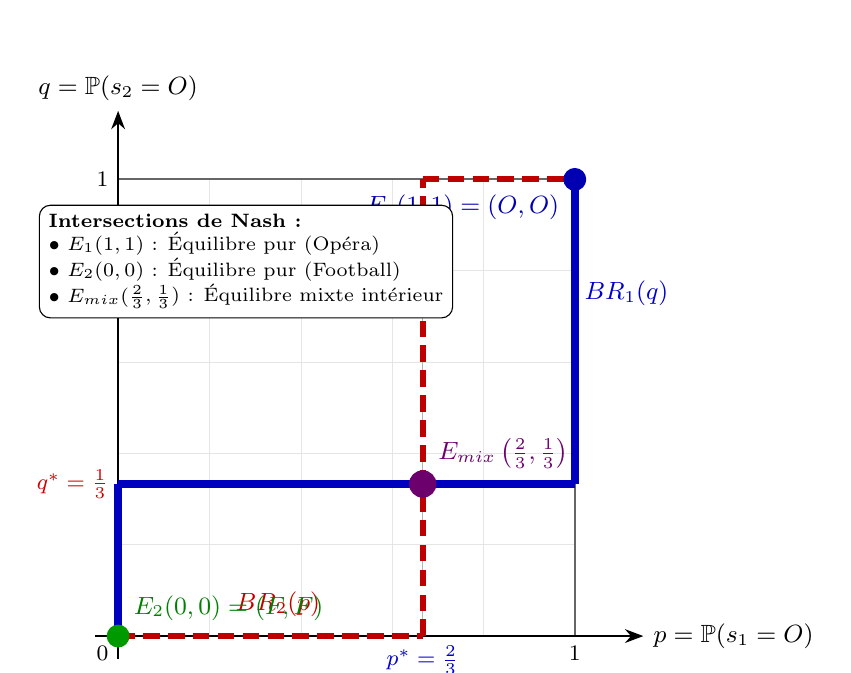
\begin{tikzpicture}[scale=5.8]
    % Cadre et grille
    \draw[step=0.2, gray!20, very thin] (0,0) grid (1,1);
    \draw[thick, black!60] (0,0) rectangle (1,1);
    
    % Axes
    \draw[->, >=Stealth, thick] (-0.05,0) -- (1.15,0) node[right, font=\small] {$p = \mathbb{P}(s_1 = O)$};
    \draw[->, >=Stealth, thick] (0,-0.05) -- (0,1.15) node[above, font=\small] {$q = \mathbb{P}(s_2 = O)$};
    
    % Graduations
    \node[below left, font=\footnotesize] at (0,0) {$0$};
    \node[below, font=\footnotesize] at (1,0) {$1$};
    \node[left, font=\footnotesize] at (0,1) {$1$};
    \node[below, blue!80!black, font=\footnotesize\bfseries] at (0.667,0) {$p^* = \frac{2}{3}$};
    \node[left, red!80!black, font=\footnotesize\bfseries] at (0,0.333) {$q^* = \frac{1}{3}$};
    
    % Lignes directrices pointillées
    \draw[dashed, gray!60] (0.667, 0) -- (0.667, 1);
    \draw[dashed, gray!60] (0, 0.333) -- (1, 0.333);
    
    % BR1(q) en Bleu continu très épais
    % Pour q in [0, 1/3[, p = 0
    \draw[blue!75!black, line width=2.8pt] (0, 0) -- (0, 0.333);
    % Pour q = 1/3, p in [0, 1]
    \draw[blue!75!black, line width=2.8pt] (0, 0.333) -- (1, 0.333);
    % Pour q in ]1/3, 1], p = 1
    \draw[blue!75!black, line width=2.8pt] (1, 0.333) -- (1, 1);
    \node[blue!80!black, font=\small\bfseries, right] at (1, 0.75) {$BR_1(q)$};
    
    % BR2(p) en Rouge tireté très épais
    % Pour p in [0, 2/3[, q = 0
    \draw[red!75!black, line width=2.2pt, dash pattern=on 6pt off 3pt] (0, 0) -- (0.667, 0);
    % Pour p = 2/3, q in [0, 1]
    \draw[red!75!black, line width=2.2pt, dash pattern=on 6pt off 3pt] (0.667, 0) -- (0.667, 1);
    % Pour p in ]2/3, 1], q = 1
    \draw[red!75!black, line width=2.2pt, dash pattern=on 6pt off 3pt] (0.667, 1) -- (1, 1);
    \node[red!75!black, font=\small\bfseries, above] at (0.35, 0.02) {$BR_2(p)$};
    
    % Points d'équilibre (Intersections)
    \fill[green!60!black] (0, 0) circle (0.025);
    \node[above right=3pt, green!50!black, font=\small\bfseries] at (0, 0) {$E_2(0, 0) = (F, F)$};
    
    \fill[blue!70!black] (1, 1) circle (0.025);
    \node[below left=3pt, blue!70!black, font=\small\bfseries] at (1, 1) {$E_1(1, 1) = (O, O)$};
    
    \fill[violet!85!black] (0.667, 0.333) circle (0.03);
    \node[above right=3pt, violet!85!black, font=\small\bfseries] at (0.667, 0.333) {$E_{mix}\left(\frac{2}{3}, \frac{1}{3}\right)$};
    
    % Légende intégrée
    \node[draw, fill=white, rounded corners, font=\scriptsize, align=left] at (0.28, 0.82) {
        \textbf{Intersections de Nash :} \\
        $\bullet$ $E_1(1,1)$ : Équilibre pur (Opéra) \\
        $\bullet$ $E_2(0,0)$ : Équilibre pur (Football) \\
        $\bullet$ $E_{mix}(\frac{2}{3}, \frac{1}{3})$ : Équilibre mixte intérieur
    };
\end{tikzpicture}
\end{center}

\newpage

%=====================================================================
% SECTION 3 : COMPARAISON ANALYTIQUE DES GAINS
%=====================================================================
\section{Comparaison Analytique des Équilibres et Défaillance de Coordination}\label{sec:comparaison}

\subsection{Calcul des gains espérés respectifs}
La consigne de départ nous invite à comparer les équilibres et leurs gains espérés respectifs. Évaluons avec précision l'utilité perçue par chaque agent dans chacune des trois configurations d'équilibre :

\begin{enumerate}[label=(\alph*),leftmargin=1.5em]
    \item \textbf{À l'équilibre pur $E_1 = (O, O)$ :}
    \begin{equation}
    u_1(E_1) = P, \qquad u_2(E_1) = Q, \qquad W(E_1) = u_1 + u_2 = P + Q.
    \end{equation}
    En valeur canonique : $u_1 = 2, u_2 = 1, W = 3$.
    
    \item \textbf{À l'équilibre pur $E_2 = (F, F)$ :}
    \begin{equation}
    u_1(E_2) = Q, \qquad u_2(E_2) = P, \qquad W(E_2) = u_1 + u_2 = P + Q.
    \end{equation}
    En valeur canonique : $u_1 = 1, u_2 = 2, W = 3$.
    
    \item \textbf{À l'équilibre mixte $E_{mix} = (p^*, q^*)$ :}
    Puisque le Joueur 1 est indifférent entre $O$ et $F$, son gain espéré peut être calculé indifféremment sur l'action $O$ :
    \[
    u_1(p^*, q^*) = u_1(O, q^*) = q^* P + (1 - q^*) N.
    \]
    En injectant l'expression de $q^* = \frac{Q - N}{P + Q - 2N}$ :
    \begin{align}
    u_1^* &= \left( \frac{Q - N}{P + Q - 2N} \right) P + \left( 1 - \frac{Q - N}{P + Q - 2N} \right) N \nonumber \\
          &= \frac{P(Q - N) + N(P + Q - 2N - Q + N)}{P + Q - 2N} \nonumber \\
          &= \frac{PQ - PN + N(P - N)}{P + Q - 2N} = \frac{PQ - PN + PN - N^2}{P + Q - 2N} \nonumber \\
          &= \frac{PQ - N^2}{P + Q - 2N}.
    \end{align}
    De façon parfaitement symétrique pour le Joueur 2 :
    \begin{equation}
    u_2^* = u_2(p^*, O) = p^* Q + (1 - p^*) N = \frac{PQ - N^2}{P + Q - 2N}.
    \end{equation}
\end{enumerate}

\begin{propbox}{Théorème 3 : Égalité et valeur des gains mixtes}
À l'équilibre de Nash en stratégies mixtes, les deux joueurs obtiennent \textbf{une espérance de gain rigoureusement identique} :
\begin{equation}\label{eq:gain_mixte_formel}
\boxed{u_1^* = u_2^* = \frac{PQ - N^2}{P + Q - 2N}}.
\end{equation}
Dans le cas canonique ($P = 2, Q = 1, N = 0$) :
\begin{equation}
u_1^* = u_2^* = \frac{2 \times 1 - 0}{2 + 1 - 0} = \frac{2}{3} \approx 0{,}667.
\end{equation}
Le bien-être social total généré par l'équilibre mixte est :
\begin{equation}
W(E_{mix}) = u_1^* + u_2^* = \frac{2(PQ - N^2)}{P + Q - 2N} \quad \xrightarrow{\text{canonique}} \quad W(E_{mix}) = \frac{4}{3} \approx 1{,}333.
\end{equation}
\end{propbox}

\subsection{Démonstration du Théorème de Défaillance de Coordination}
Comparons à présent formellement ce gain mixte $u_{mix}^*$ aux gains obtenus lors des coordinations pures :

\begin{propbox}{Théorème 4 : Défaillance de coordination (\emph{Coordination Failure})}
Pour tout jeu de la Bataille des Sexes vérifiant les hypothèses naturelles $P > Q > N \ge 0$, le gain espéré à l'équilibre mixte est \textbf{strictement inférieur au pire des gains obtenus en cas de coordination pure} :
\begin{equation}
\boxed{u_{mix}^* < Q < P}.
\end{equation}
\end{propbox}

\begin{proof}
Calculons la différence exacte $\Delta = u_{mix}^* - Q$ :
\begin{align}
\Delta &= \frac{PQ - N^2}{P + Q - 2N} - Q \nonumber \\
       &= \frac{PQ - N^2 - Q(P + Q - 2N)}{P + Q - 2N} \nonumber \\
       &= \frac{PQ - N^2 - PQ - Q^2 + 2QN}{P + Q - 2N} \nonumber \\
       &= \frac{- (Q^2 - 2QN + N^2)}{P + Q - 2N} \nonumber \\
       &= - \frac{(Q - N)^2}{P + Q - 2N}.
\end{align}
Puisque par hypothèse $Q > N$, on a $(Q - N)^2 > 0$. De plus, $P > Q > N \implies P - N > 0$ et $Q - N > 0$, donc le dénominateur vérifie :
\[
P + Q - 2N = (P - N) + (Q - N) > 0.
\]
Le quotient $\frac{(Q - N)^2}{P + Q - 2N}$ est donc strictement positif, ce qui implique que son opposé est strictement négatif :
\[
\Delta = u_{mix}^* - Q < 0 \iff u_{mix}^* < Q.
\]
Comme $Q < P$, on en déduit immédiatement la double inégalité stricte :
\[
u_{mix}^* < Q < P. \qedhere
\]
\end{proof}

\begin{rembox}{Interprétation économique majeure}
Ce théorème met en évidence le \textbf{coût social dramatique de l'indétermination stratégique} :
\begin{itemize}[leftmargin=1.5em]
    \item Même si un joueur est contraint d'accepter son issue la moins préférée (gain $Q = 1$), il se porte \textbf{strictement mieux} qu'en recourant à la randomisation mixte (gain $2/3 \approx 0{,}67$).
    \item L'équilibre mixte, bien qu'il rétablisse une forme de symétrie procédurale entre les agents ($u_1^* = u_2^*$), détruit massivement de l'utilité collective par le risque permanent de désaccord.
\end{itemize}
\end{rembox}

\subsection{Quantification probabiliste du risque de désaccord}
Sous l'équilibre mixte canonique, les choix des deux joueurs étant stochastiquement indépendants, la probabilité d'occurrence conjointe de chacune des 4 cellules de la matrice s'établit comme suit :
\begin{center}
\small
\renewcommand{\arraystretch}{1.3}
\begin{tabular}{lcc}
\toprule
\textbf{Issue $(s_1, s_2)$} & \textbf{Probabilité théorique} & \textbf{Valeur numérique} \\
\midrule
$(O, O)$ -- Coordination sur Opéra & $p^* q^* = \frac{2}{3} \times \frac{1}{3} = \frac{2}{9}$ & $\approx 22{,}22\%$ \\
$(F, F)$ -- Coordination sur Football & $(1-p^*)(1-q^*) = \frac{1}{3} \times \frac{2}{3} = \frac{2}{9}$ & $\approx 22{,}22\%$ \\
$(O, F)$ -- Désaccord (J1 à Opéra, J2 à Football) & $p^*(1-q^*) = \frac{2}{3} \times \frac{2}{3} = \frac{4}{9}$ & $\approx 44{,}44\%$ \\
$(F, O)$ -- Désaccord (J1 à Football, J2 à Opéra) & $(1-p^*)q^* = \frac{1}{3} \times \frac{1}{3} = \frac{1}{9}$ & $\approx 11{,}11\%$ \\
\bottomrule
\end{tabular}
\end{center}

La probabilité cumulée de \textbf{réussite de la coordination} est :
\begin{equation}
\mathbb{P}(\text{Succès}) = \mathbb{P}(O, O) + \mathbb{P}(F, F) = \frac{2}{9} + \frac{2}{9} = \frac{4}{9} \approx 44{,}44\%.
\end{equation}
La probabilité cumulée d'\textbf{échec de coordination (désaccord)} atteint :
\begin{equation}
\mathbb{P}(\text{Échec}) = \mathbb{P}(O, F) + \mathbb{P}(F, O) = \frac{4}{9} + \frac{1}{9} = \frac{5}{9} \approx \mathbf{55{,}56\%}.
\end{equation}

\textbf{Constat statistique accablant :} lorsque deux décideurs parfaitement rationnels appliquent la prescription mixte de Nash, ils se retrouvent \textbf{séparés et bredouilles dans plus d'un cas sur deux} ($55{,}56\%$) !

\subsection{Évaluation du Prix de l'Anarchie (PoA) et du Prix de la Stabilité (PoS)}
En théorie algorithmique des jeux (Nisan, Roughgarden, Tardos \& Vazirani, 2007), deux métriques standard permettent de quantifier l'inefficacité d'un système décentralisé non coordonné :

\begin{propbox}{Définition 2 : Prix de l'Anarchie et Prix de la Stabilité}
Soit $\mathcal{E}$ l'ensemble des équilibres de Nash du jeu, et $W(s) = u_1(s) + u_2(s)$ la fonction de bien-être social utilitariste.
\begin{equation}
\text{Price of Anarchy (PoA)} = \frac{\max_{s \in S} W(s)}{\min_{s^* \in \mathcal{E}} W(s^*)},
\end{equation}
\begin{equation}
\text{Price of Stability (PoS)} = \frac{\max_{s \in S} W(s)}{\max_{s^* \in \mathcal{E}} W(s^*)}.
\end{equation}
\end{propbox}

Dans notre jeu de la Bataille des Sexes :
\begin{itemize}[leftmargin=1.5em]
    \item L'optimum social est atteint sur l'un ou l'autre des équilibres purs : $W_{opt} = P + Q = 3$.
    \item Le meilleur équilibre de Nash offre un bien-être social de $W = 3$. Donc :
    \begin{equation}
    \text{PoS} = \frac{3}{3} = \mathbf{1{,}00}.
    \end{equation}
    \item Le pire équilibre de Nash est l'équilibre mixte, avec $W(E_{mix}) = 4/3$. Par conséquent :
    \begin{equation}
    \text{PoA} = \frac{3}{4/3} = \frac{9}{4} = \mathbf{2{,}25}.
    \end{equation}
\end{itemize}

Ce PoA de $2{,}25$ signifie que l'absence de mécanisme de coordination déterministe peut dégrader l'efficacité sociale globale d'un facteur supérieur à 2.

\newpage

%=====================================================================
% SECTION 4 : CRITIQUES ÉPISTÉMIQUES ET NOUVEAUX CONCEPTS
%=====================================================================
\section{Critiques Épistémiques et Concepts Alternatifs de Solution}\label{sec:epistemique}

\subsection{La critique épistémique sous CKR (Léo Gerville-Réache, HAL 2017)}
Dans une étude stimulante consacrée aux fondements cognitifs de la théorie des jeux (*L'issue de la Bataille des Sexes sous CKR*, 2017), Léo Gerville-Réache (Université de Bordeaux) remet en cause la validité de l'équilibre mixte sous l'hypothèse canonique de \textbf{Connaissance Commune de la Rationalité} (\emph{Common Knowledge of Rationality} -- CKR).

Le raisonnement orthodoxe de Nash affirme que l'époux joue Foot avec probabilité $2/3$ car il sait que son épouse joue Foot avec probabilité $1/3$ pour le rendre indifférent. Or, comme le souligne Bernard Guerrien (2002) :
\begin{quote}
\textit{« Si je suis certain que mon épouse choisira le football avec probabilité $1/3$, je suis rigoureusement indifférent entre l'opéra et le football, car les deux me rapportent exactement une espérance de $2/3$. Mais alors, pourquoi cette indifférence absolue devrait-elle me dicter de choisir précisément le football avec une probabilité de $2/3$ plutôt que $1/2$ ou n'importe quelle autre fréquence ? »}
\end{quote}

Pour contourner cette incohérence décisionnelle, l'équilibre de Nash impose de facto une privation réciproque de libre arbitre : chaque joueur est contraint d'adopter le mélange requis pour soutenir l'équilibre de l'autre. Dès lors que l'on rejette cette fiction d'absence de choix autonome, d'autres concepts de solution s'imposent naturellement.

\subsection{L'approche de sécurité : Stratégie Maximin de von Neumann}
Considérons l'attitude d'un joueur prudent qui refuse de spéculer sur la bienveillance ou la coordination de l'autre et cherche à se garantir un niveau de paiement minimal :

\begin{propbox}{Définition 3 : Stratégie de sécurité Maximin}
La stratégie de sécurité du Joueur 1 maximise son gain minimal garanti face au pire comportement possible du Joueur 2 :
\begin{equation}
\max_{p \in [0, 1]} \min_{q \in [0, 1]} u_1(p, q).
\end{equation}
\end{propbox}

Calculons cette stratégie pour le Joueur 1 :
\begin{itemize}[leftmargin=1.5em]
    \item Si le Joueur 2 joue $O$ ($q = 1$), le gain du Joueur 1 est $2p$.
    \item Si le Joueur 2 joue $F$ ($q = 0$), le gain du Joueur 1 est $1 - p$.
\end{itemize}
Le pire gain possible face à une action pure adverse est donc $\min(2p, 1 - p)$. Cette fonction en toit est maximisée au point d'égalisation :
\[
2p = 1 - p \iff 3p = 1 \implies \boxed{p_{sec} = \frac{1}{3}}.
\]
Le niveau de sécurité garanti est alors :
\begin{equation}
v_1 = 2 \times \frac{1}{3} = 1 - \frac{1}{3} = \mathbf{\frac{2}{3}}.
\end{equation}
De façon symétrique, pour le Joueur 2 :
\[
q \cdot 1 = (1 - q) \cdot 2 \iff 3q = 2 \implies \boxed{q_{sec} = \frac{2}{3}}, \qquad v_2 = \mathbf{\frac{2}{3}}.
\]

\begin{propbox}{Théorème 5 : Équivalence frappante Nash mixte / Sécurité}
Le niveau de sécurité garanti par la stratégie de précaution Maximin est \textbf{rigoureusement égal au gain espéré du Nash mixte} :
\begin{equation}
v_1 = v_2 = u_1^* = u_2^* = \frac{2}{3}.
\end{equation}
\end{propbox}
Ce théorème révèle un paradoxe majeur : \textbf{le jeu interactif mixte de Nash ne rapporte strictement rien de plus aux agents qu'une attitude de défiance totale} où chaque joueur considérerait son partenaire comme un ennemi destructeur cherchant à minimiser son utilité !

\subsection{L'issue symétrique collective sous CKR}
Sous CKR, dans un jeu symétrique sans communication, la rationalité collective impose une symétrie parfaite de raisonnement : les deux conjoints doivent adopter la même probabilité $p$ de choisir leur activité préférée respective.
Dans ce cadre, la probabilité que les deux se coordonnent sur l'opéra est $p(1-p)$, et sur le football $(1-p)p$. L'espérance de gain symétrique s'écrit :
\begin{equation}
u_{sym}(p) = p(1-p) \cdot 2 + (1-p)p \cdot 1 = 3p(1-p).
\end{equation}
Pour maximiser cette fonction quadratique concave sur $[0, 1]$ :
\[
\frac{d u_{sym}}{dp} = 3(1 - 2p) = 0 \implies \boxed{p_{CKR}^* = \frac{1}{2}}.
\]
Le gain espéré maximal sous raisonnement symétrique atteint :
\begin{equation}
u_{sym}\left(\frac{1}{2}\right) = 3 \times \frac{1}{2} \times \frac{1}{2} = \mathbf{\frac{3}{4} = 0{,}75 > 0{,}667}.
\end{equation}
Le choix de l'équiprobabilité ($p=1/2$) surmonte l'équilibre de Nash mixte en augmentant le gain de chaque agent de $12{,}5\%$.

\subsection{L'Équilibre Corrélé de Robert Aumann (1974)}
Pour réconcilier efficacité maximale ($W = 3$) et équité distributionnelle parfaite ($u_1 = u_2$), Robert Aumann (Prix Nobel 2005) a formulé le concept d'\textbf{équilibre corrélé} :

\begin{propbox}{Définition 4 : Équilibre Corrélé (Aumann, 1974)}
Soit une distribution de probabilité conjointe $z = (z_{OO}, z_{OF}, z_{FO}, z_{FF}) \in \Delta(S_1 \times S_2)$. Un médiateur ou un mécanisme public tire un profil d'actions $(s_1, s_2)$ selon $z$ et transmet confidentiellement à chaque joueur $i$ son action recommandée $s_i$.
La distribution $z$ est un équilibre corrélé si et seulement si aucun joueur n'a intérêt à dévier de la recommandation reçue :
\begin{equation}
\sum_{s_{-i} \in S_{-i}} z(s_i, s_{-i}) \left[ u_i(s_i, s_{-i}) - u_i(s_i', s_{-i}) \right] \ge 0, \quad \forall i, \ \forall s_i, s_i' \in S_i.
\end{equation}
\end{propbox}

Pour la Bataille des Sexes, supposons que les deux conjoints conviennent de regarder un signal public équilibré (par exemple un lancer de pièce de monnaie équitable avant de partir) :
\begin{itemize}[leftmargin=1.5em]
    \item Si « Pile » : le dispositif recommande $(O, O)$ (probabilité $1/2$).
    \item Si « Face » : le dispositif recommande $(F, F)$ (probabilité $1/2$).
    \item Les issues de désaccord reçoivent une probabilité nulle : $z_{OF} = z_{FO} = 0$.
\end{itemize}

Vérifions les contraintes d'incitation (absence de déviation unilatérale) :
\begin{itemize}[leftmargin=1.5em]
    \item Si le Joueur 1 reçoit la consigne $O$, il sait que le Joueur 2 a reçu $O$. S'il obéit, il gagne 2. S'il dévie vers $F$, il gagne 0. $2 \ge 0$ : aucune déviation profitable.
    \item Si le Joueur 1 reçoit la consigne $F$, il sait que le Joueur 2 a reçu $F$. S'il obéit, il gagne 1. S'il dévie vers $O$, il gagne 0. $1 \ge 0$ : aucune déviation profitable.
\end{itemize}

L'espérance de gain obtenue par chaque agent est :
\begin{equation}
u_1^{CE} = u_2^{CE} = \frac{1}{2} \times 2 + \frac{1}{2} \times 1 = \mathbf{\frac{3}{2} = 1{,}50}.
\end{equation}
Cet équilibre corrélé réalise la synthèse parfaite :
\begin{enumerate}[label=(\roman*)]
    \item \textbf{Efficacité totale} : aucun gaspillage de coordination ($\mathbb{P}(\text{Succès}) = 100\%$, $W = 3$).
    \item \textbf{Équité absolue} : symétrie parfaite des gains sans favoritisme ($u_1 = u_2 = 1{,}5$).
    \item \textbf{Pareto-dominance stricte} : il domine strictement le Nash mixte ($1{,}5 > 0{,}667$) et l'issue CKR ($1{,}5 > 0{,}75$).
\end{enumerate}

\newpage

%=====================================================================
% SECTION 5 : SÉLECTION D'ÉQUILIBRE ET POINTS FOCAUX
%=====================================================================
\section{Sélection d'Équilibre et Points Focaux de Schelling}\label{sec:schelling}

\subsection{La théorie des points focaux de Thomas Schelling (1960)}
Dans son chef-d'\oe uvre *The Strategy of Conflict* (1960), Thomas Schelling (Prix Nobel 2005) introduit une rupture épistémologique majeure : lorsque la structure mathématique abstraite d'un jeu présente plusieurs équilibres équivalents ou symétriques, les acteurs humains réels parviennent pourtant à converger spontanément avec une régularité impressionnante grâce à des repères qualitatifs hors-modèle :

\begin{propbox}{Définition 5 : Point focal (Schelling Point)}
Un \textbf{point focal} est une issue d'équilibre qui possède une \textbf{saillance psychologique, culturelle, linguistique ou contextuelle} distincte. Cette saillance permet aux agents d'aligner leurs anticipations mutuelles d'ordre supérieur : chaque joueur choisit cet équilibre car il anticipe que l'autre joueur anticipe qu'il va le choisir.
\end{propbox}

Schelling illustre ce principe par des expériences empiriques célèbres :
\begin{itemize}[leftmargin=1.5em]
    \item \textbf{Le rendez-vous à New York} : demandez à deux personnes de se retrouver à New York un jour précis sans pouvoir communiquer. Bien qu'il existe des millions de lieux et d'heures possibles, une majorité écrasante converge spontanément sur le kiosque d'information de \emph{Grand Central Terminal à midi pile}.
    \item \textbf{Le partage de 100 dollars} : deux individus doivent proposer un partage sans négocier ; s'ils demandent ensemble plus de 100 \$, ils ne reçoivent rien. La solution focale universelle est le partage équitable 50/50.
\end{itemize}

Dans la Bataille des Sexes, en l'absence de conventions externes, les deux équilibres $(O,O)$ et $(F,F)$ sont symétriques du point de vue de la structure pure des gains. Dès lors, la sélection du point focal dépendra d'indices contextuels :
\begin{itemize}[leftmargin=1.5em]
    \item \textbf{Précédents historiques et habitudes} : si le couple est allé au football lors de la dernière sortie, une norme sociale d'alternance désignera l'opéra comme point focal naturel.
    \item \textbf{Célébrations et contextes spécifiques} : si la soirée coïncide avec l'anniversaire de l'épouse, l'opéra devient l'issue saillante évidente pour les deux joueurs.
\end{itemize}

\subsection{Mécanismes stratégiques et dynamiques de sélection}

\subsubsection{1. Communication préalable non contraignante (\emph{Cheap Talk})}
Selon les modèles de Vincent Crawford et Joel Sobel (1982) et Joseph Farrell (1987) :
\begin{itemize}[leftmargin=1.5em]
    \item \textbf{Annonce unilatérale} : si l'un des joueurs a l'opportunité d'envoyer un message avant le choix (« Je me rends à l'Opéra ce soir »), ce message n'a aucun coût contractuel direct (\emph{cheap talk}), mais il est \textbf{stratégiquement crédible} car le joueur récepteur a tout intérêt à s'y conformer pour empocher $Q=1$ plutôt que $N=0$. L'émetteur s'empare ainsi de l'avantage du premier déclarant.
    \item \textbf{Annonces bilatérales simultanées} : si les deux crient simultanément leur souhait, le conflit de coordination persiste et des signaux contradictoires réintroduisent le risque de désaccord.
\end{itemize}

\subsubsection{2. Engagement irréversible et leadership de Stackelberg}
Dans le Chapitre 15 du manuel de cours (*Shutdown - Le jeu de la guerre des sexes*), l'engagement stratégique est mis en scène de façon magistrale :
\begin{quote}
\textit{Lucie achète à l'avance un billet d'opéra non remboursable et très coûteux, puis elle envoie une confirmation formelle à Charles. En posant cet acte irréversible, elle détruit volontairement sa propre option de pouvoir aller au football sans subir une perte immense.}
\end{quote}

Cette transformation convertit le jeu simultané en un jeu séquentiel à deux étapes :
\begin{center}
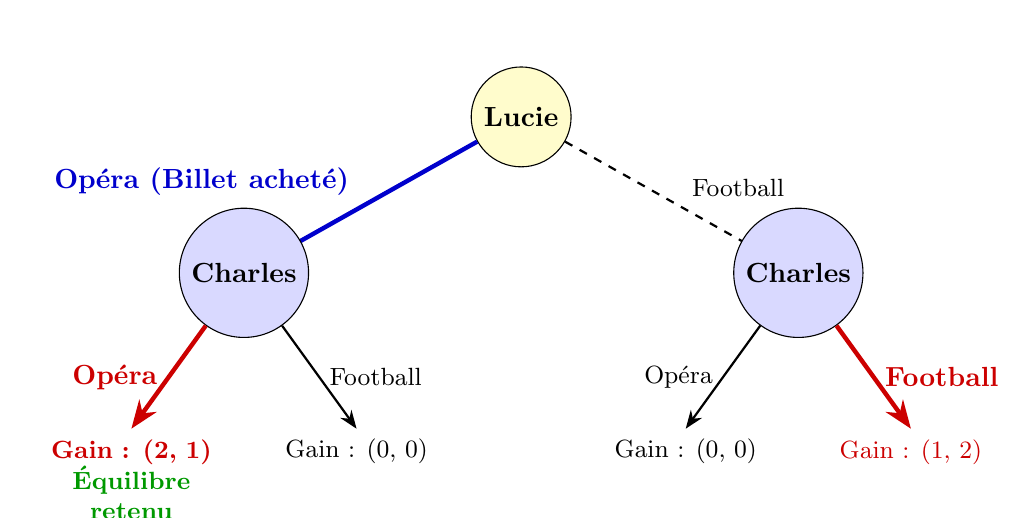
\begin{tikzpicture}[scale=1.1, >=Stealth, every node/.style={font=\small}]
    % Arbre séquentiel TikZ
    \node[draw, circle, fill=yellow!20, font=\bfseries] (Root) at (0, 0) {Lucie};
    
    \coordinate (L_Op) at (-3.2, -1.8);
    \coordinate (L_Ft) at (3.2, -1.8);
    
    \draw[->, ultra thick, blue!80!black] (Root) -- (L_Op) node[midway, above left, font=\bfseries] {Opéra (Billet acheté)};
    \draw[->, thick, dashed] (Root) -- (L_Ft) node[midway, above right] {Football};
    
    \node[draw, circle, fill=blue!15, font=\bfseries] (NodeC1) at (L_Op) {Charles};
    \node[draw, circle, fill=blue!15, font=\bfseries] (NodeC2) at (L_Ft) {Charles};
    
    % Branches Charles
    \draw[->, ultra thick, red!80!black] (NodeC1) -- (-4.5, -3.6) node[midway, left, font=\bfseries] {Opéra} node[below, text width=2.4cm, align=center] {\textbf{Gain : (2, 1)}\\\textcolor{green!60!black}{\textbf{Équilibre retenu}}};
    \draw[->, thick] (NodeC1) -- (-1.9, -3.6) node[midway, right] {Football} node[below] {Gain : (0, 0)};
    
    \draw[->, thick] (NodeC2) -- (1.9, -3.6) node[midway, left] {Opéra} node[below] {Gain : (0, 0)};
    \draw[->, ultra thick, red!80!black] (NodeC2) -- (4.5, -3.6) node[midway, right, font=\bfseries] {Football} node[below] {Gain : (1, 2)};
\end{tikzpicture}
\end{center}

Par \textbf{induction à rebours} (*backward induction*) :
\begin{itemize}[leftmargin=1.5em]
    \item Face à l'engagement visible de Lucie à l'opéra, Charles compare son gain en la rejoignant ($u_C = 1$) à son gain en partant seul au stade ($u_C = 0$). Sa meilleure réponse rationnelle est de capituler et d'aller à l'opéra.
    \item Lucie anticipe cette capitulation rationnelle : en achetant le billet, elle s'assure un gain maximal de 2 (au lieu de 1).
\end{itemize}
Cet exemple valide l'axiome paradoxal de Schelling : \textbf{en théorie des jeux, restreindre sa propre liberté d'action renforce son pouvoir de négociation}.

\subsubsection{3. Répétition temporelle et Théorème Folk (Turn-Taking)}
Dans une interaction répétée à horizon infini où les joueurs actualisent leurs gains futurs avec un facteur d'escompte $\delta \in ]0, 1[$, le \textbf{théorème Folk} prouve qu'une convention sociale d'alternance (« Opéra les semaines paires, Football les semaines impaires ») constitue un équilibre parfait en sous-jeux stable, soutenu par des stratégies de déclic (*grim trigger*). Cette convention interne émule parfaitement l'équilibre corrélé sans nécessiter d'arbitre extérieur.

\subsection{Dynamique évolutive du réplicateur (Stabilité locale)}
En biologie théorique et en économie comportementale (Maynard Smith, 1982), la dynamique du réplicateur modélise l'évolution de la proportion de chaque stratégie au sein de populations en interaction aléatoire.
Considérons deux populations :
\begin{itemize}[leftmargin=1.5em]
    \item Population 1 (Joueurs 1) : proportion $p$ jouant $O$, proportion $1-p$ jouant $F$.
    \item Population 2 (Joueurs 2) : proportion $q$ jouant $O$, proportion $1-q$ jouant $F$.
\end{itemize}

Le système différentiel continu du réplicateur s'écrit :
\begin{align}
\dot{p} &= p \cdot \left[ u_1(O, q) - \bar{u}_1(p, q) \right] = p(1 - p) \left[ u_1(O, q) - u_1(F, q) \right], \\
\dot{q} &= q \cdot \left[ u_2(p, O) - \bar{u}_2(p, q) \right] = q(1 - q) \left[ u_2(p, O) - u_2(p, F) \right].
\end{align}

Pour le cas canonique ($P = 2, Q = 1, N = 0$) :
\begin{equation}\label{eq:replicator_system}
\begin{cases}
\dot{p} = p(1 - p)(3q - 1), \\
\dot{q} = q(1 - q)(3p - 2).
\end{cases}
\end{equation}

Les points stationnaires ($\dot{p} = 0, \dot{q} = 0$) sur $[0, 1]^2$ sont :
\begin{enumerate}[label=(\roman*)]
    \item Les 4 coins du carré unitaire : $(0, 0)$, $(1, 1)$, $(0, 1)$, $(1, 0)$.
    \item L'équilibre de Nash mixte intérieur : $(p^*, q^*) = \left(\frac{2}{3}, \frac{1}{3}\right)$.
\end{enumerate}

Calculons la matrice jacobienne $J(p, q)$ du système linéarisé :
\begin{equation}
J(p, q) = \begin{pmatrix}
\frac{\partial \dot{p}}{\partial p} & \frac{\partial \dot{p}}{\partial q} \\
\frac{\partial \dot{q}}{\partial p} & \frac{\partial \dot{q}}{\partial q}
\end{pmatrix}
= \begin{pmatrix}
(1 - 2p)(3q - 1) & 3p(1 - p) \\
3q(1 - q) & (1 - 2q)(3p - 2)
\end{pmatrix}.
\end{equation}

Évaluons cette jacobienne au point intérieur mixte $(p^*, q^*) = \left(\frac{2}{3}, \frac{1}{3}\right)$ :
\begin{itemize}[leftmargin=1.5em]
    \item Comme $3q^* - 1 = 0$ et $3p^* - 2 = 0$, les termes diagonaux s'annulent rigoureusement :
    \[
    J_{11} = 0, \qquad J_{22} = 0.
    \]
    \item Les termes hors-diagonaux valent :
    \[
    J_{12} = 3 \times \frac{2}{3} \times \left(1 - \frac{2}{3}\right) = 2 \times \frac{1}{3} = \frac{2}{3},
    \]
    \[
    J_{21} = 3 \times \frac{1}{3} \times \left(1 - \frac{1}{3}\right) = 1 \times \frac{2}{3} = \frac{2}{3}.
    \]
\end{itemize}

La jacobienne s'écrit donc :
\begin{equation}
J\left(\frac{2}{3}, \frac{1}{3}\right) = \begin{pmatrix}
0 & \frac{2}{3} \\
\frac{2}{3} & 0
\end{pmatrix}.
\end{equation}

Déterminons ses valeurs propres par l'équation caractéristique $\det(J - \lambda I) = 0$ :
\[
\lambda^2 - \left(\frac{2}{3}\right)^2 = 0 \implies \lambda_1 = +\frac{2}{3}, \quad \lambda_2 = -\frac{2}{3}.
\]
Le déterminant de la jacobienne est strictement négatif :
\begin{equation}
\det(J) = - \frac{4}{9} < 0.
\end{equation}

\begin{propbox}{Théorème 6 : Instabilité structurelle de l'équilibre mixte (Point-selle)}
Puisque les valeurs propres sont réelles et de signes strictement opposés ($\lambda_1 > 0$ et $\lambda_2 < 0$), l'équilibre mixte de Nash est un \textbf{point-selle hyperbolique dynamiquement instable}.
\textbf{Conséquences dynamiques :}
\begin{enumerate}[label=(\roman*)]
    \item L'équilibre mixte n'est jamais une Stratégie Évolutionnairement Stable (ESS au sens de John Maynard Smith).
    \item Toute perturbation stochastique ou bruit environnemental infinitésimal écarte irréversiblement la population de $(2/3, 1/3)$ et la précipite vers l'un des deux attracteurs purs stables : soit $(O, O)$ (si $p > 2/3$ et $q > 1/3$), soit $(F, F)$ (si $p < 2/3$ et $q < 1/3$).
\end{enumerate}
\end{propbox}

Ce résultat confirme que dans les systèmes vivants et les marchés économiques, les populations \textbf{ne restent jamais à l'équilibre mixte} : elles basculent spontanément vers l'un des deux régimes de coordination pure.

\newpage

%=====================================================================
% SECTION 6 : APPLICATIONS RÉELLES ET CAS CONCRETS
%=====================================================================
\section{Applications Réelles et Recherche Opérationnelle}\label{sec:applications}

\subsection{Guerres de standards et normes industrielles}
Le jeu de la Bataille des Sexes constitue le cadre analytique de référence pour comprendre la compétition technologique entre formats incompatibles (Arthur, 1989 ; Shapiro \& Varian, 1999) :

\begin{enumerate}[label=(\alph*),leftmargin=1.5em]
    \item \textbf{La guerre des magnétoscopes (1976--1988) : VHS contre Betamax}
    Sony a développé le format Betamax (qualité vidéo supérieure, cassettes plus compactes, gain $P$ pour Sony). JVC a conçu le format VHS (capacité d'enregistrement plus longue, gain $P$ pour JVC).
    Pour les consommateurs et les studios hollywoodiens, le pire résultat était la coexistence durable de deux formats incompatibles divisant le marché (désaccord $N = 0$). 
    JVC a emporté la bataille en créant un \textbf{point focal massif} via une politique agressive de licences ouvertes concédées à tous les fabricants mondiaux (Matsushita, Philips, Thomson), saturant ainsi le réseau de distribution.
    
    \item \textbf{La guerre de la Haute Définition (2006--2008) : Blu-ray contre HD-DVD}
    Sony (Blu-ray) affrontait Toshiba (HD-DVD). Les deux formats étaient technologiquement proches. Le verrouillage s'est brisé en janvier 2008 grâce à un \textbf{engagement unilatéral irréversible} : le studio Warner Bros a annoncé qu'il abandonnait le HD-DVD pour publier exclusivement en Blu-ray. Cette annonce a servi de signal focal immédiat, provoquant le ralliement de toute la chaîne de valeur et la capitulation de Toshiba un mois plus tard.
    
    \item \textbf{Le connecteur universel USB-C imposé par l'Union Européenne}
    Face à la persistance d'une incompatibilité coûteuse entre Apple (port propriétaire Lightning) et l'écosystème Android/PC (USB-C), la Commission Européenne a agi comme une autorité exogène imposant un \textbf{point focal réglementaire obligatoire} par directive européenne, éliminant définitivement le coût social du désaccord pour les consommateurs.
\end{enumerate}

\subsection{Négociations politiques et blocages budgétaires (\emph{Government Shutdown})}
Dans le Chapitre 15 du manuel de cours (*Shutdown - Le jeu de la guerre des sexes*), le modèle est appliqué au bras de fer institutionnel américain entre Démocrates et Républicains :
\begin{itemize}[leftmargin=1.5em]
    \item Le vote du budget fédéral exige l'approbation conjointe de la Chambre des représentants et du Sénat.
    \item Les Démocrates souhaitent prioriser les dépenses sociales et de transition écologique ($P$ pour eux, $Q$ pour l'opposition).
    \item Les Républicains souhaitent couper les impôts et restreindre les budgets fédéraux ($P$ pour eux, $Q$ pour l'opposition).
    \item Si aucun accord n'intervient à l'échéance légale, l'État fédéral entre en \emph{shutdown} : fermeture des parcs nationaux, chômage technique pour des centaines de milliers de fonctionnaires, paralysie administrative et pertes économiques massives (issue de désaccord $(0, 0)$).
\end{itemize}
L'issue de ce jeu de négociation extrême est invariablement déterminée par la \textbf{crédibilité de la menace} : le camp politique capable de convaincre l'opinion publique et son adversaire de son intransigeance totale contraint l'autre camp à céder pour éviter la catastrophe nationale.

\subsection{Sélection technologique d'entreprise : Le problème MAC vs CAM}
Dans les exercices de travaux dirigés de Master RO (notamment le problème de la forme extensive, page 33 du guide), deux entreprises partenaires doivent choisir une plate-forme de fabrication assistée par ordinateur : MAC ou CAM.
\begin{itemize}[leftmargin=1.5em]
    \item Si les deux optent pour MAC : gains $(200, 600)$.
    \item Si les deux optent pour CAM : gains $(600, 200)$.
    \item Si elles choisissent des plates-formes divergentes : gains $(100, 100)$ en raison de l'incompatibilité des fichiers de conception.
\end{itemize}
En forme séquentielle, l'entreprise pionnière qui déploie ses serveurs et forme son personnel en premier capture la rente de leadership (gain 600), obligeant son sous-traitant à s'aligner sur son écosystème.

\newpage

%=====================================================================
% SECTION 7 : SYNTHÈSE ET VALIDATION ALGORITHMIQUE
%=====================================================================
\section{Synthèse Comparative et Validation Algorithmique}\label{sec:bilan}

\subsection{Tableau synoptique comparatif de tous les concepts de solution}
Le tableau ci-dessous récapitule l'ensemble des grandeurs théoriques et numériques obtenues pour le jeu canonique ($P = 2, Q = 1, N = 0$) :

\begin{center}
\renewcommand{\arraystretch}{1.3}
\begin{tabular}{lcccccc}
\toprule
\textbf{Concept de Solution} & $\mathbf{s_1}$ & $\mathbf{s_2}$ & $\mathbf{u_1}$ & $\mathbf{u_2}$ & $\mathbf{W_{tot}}$ & \textbf{Taux Coord.} \\
\midrule
Équilibre Pur 1 ($E_1$) & $O$ & $O$ & $2{,}00$ & $1{,}00$ & $3{,}00$ & $100\%$ \\
Équilibre Pur 2 ($E_2$) & $F$ & $F$ & $1{,}00$ & $2{,}00$ & $3{,}00$ & $100\%$ \\
\textbf{Équilibre Mixte Nash} & $p^*=2/3$ & $q^*=1/3$ & $\mathbf{0{,}67}$ & $\mathbf{0{,}67}$ & $\mathbf{1{,}33}$ & $\mathbf{44{,}4\%}$ \\
Stratégie de Sécurité (Maximin) & $p=1/3$ & $q=2/3$ & $0{,}67$ & $0{,}67$ & $1{,}33$ & $44{,}4\%$ \\
Issue Symétrique CKR (HAL 2017) & $p=1/2$ & $p=1/2$ & $0{,}75$ & $0{,}75$ & $1{,}50$ & $50{,}0\%$ \\
\textbf{Équilibre Corrélé (Aumann)} & Signal & $50/50$ & $\mathbf{1{,}50}$ & $\mathbf{1{,}50}$ & $\mathbf{3{,}00}$ & $\mathbf{100\%}$ \\
Alternance Répétée (Folk) & Pair & Impair & $1{,}50$ & $1{,}50$ & $3{,}00$ & $100\%$ \\
\bottomrule
\end{tabular}
\end{center}

\subsection{Architecture et validation du module Python}
L'ensemble de nos démonstrations théoriques a fait l'objet d'une implémentation numérique complète dans le fichier \texttt{projet8\_coordination.py}. Ce script intègre :
\begin{enumerate}[label=(\arabic*),leftmargin=1.5em]
    \item La classe \texttt{BattleOfTheSexesGame} paramétrable par $(P, Q, N)$ ;
    \item La détection exacte des équilibres purs par opérateur de meilleure réponse ;
    \item Le calcul analytique fractionnaire exact via la bibliothèque standard \texttt{fractions.Fraction} ;
    \item La preuve formelle du théorème de sous-optimalité via le moteur symbolique \texttt{sympy} ;
    \item La résolution de l'Équilibre Corrélé par Programmation Linéaire sous solveur \texttt{scipy.optimize}\allowbreak\texttt{.linprog} (méthode HiGHS dual-simplex) ;
    \item Le calcul de la jacobienne et des valeurs propres de la dynamique du réplicateur ;
    \item Un simulateur Monte-Carlo à $50\,000$ itérations générant les statistiques empiriques de coordination.
\end{enumerate}

\begin{verifbox}
La suite de tests automatisée intégrée valide \textbf{19 assertions mathématiques exactes} avec un taux de réussite de $100\%$ :
\begin{itemize}[leftmargin=1.5em]
    \item Existence et localisation exacte des deux équilibres purs : $E_1=(O, O)$ et $E_2=(F, F)$.
    \item Calcul exact des probabilités mixtes : $p^* = 2/3$ et $q^* = 1/3$.
    \item Gains espérés mixtes exacts : $u_1^* = u_2^* = 2/3 < Q = 1$.
    \item Preuve symbolique automatisée : $\text{diff} = -(Q - N)^2 / (P + Q - 2N) < 0$.
    \item Probabilité d'échec de coordination : $5/9 \approx 55{,}56\%$.
    \item Prix de l'Anarchie ($2{,}25$) et Prix de la Stabilité ($1{,}00$).
    \item Égalité du gain de sécurité et du gain mixte ($v = 2/3$).
    \item Gain optimal sous CKR symétrique ($3/4 = 0{,}75$).
    \item Équilibre corrélé optimal : gains $(1{,}50, 1{,}50)$ et bien-être social maximal de $3{,}00$.
    \item Déterminant jacobien au point mixte : $\det(J) = -4/9 < 0$ (point-selle instable).
\end{itemize}
\end{verifbox}

\subsection{Le simulateur interactif : \texttt{dashboard\_coordination.html}}
Pour permettre une exploration pédagogique et visuelle immédiate, une interface web interactive autonome a été développée :
\begin{itemize}[leftmargin=1.5em]
    \item \textbf{Paramétrage instantané} : saisie en temps réel des valeurs $P, Q, N$ avec recalcul immédiat des équilibres ;
    \item \textbf{Tracé SVG interactif} : affichage en direct des courbes $BR_1(q)$ et $BR_2(p)$ et déplacement dynamique du point mixte ;
    \item \textbf{Simulateur Monte-Carlo intégré} : exécution dans le navigateur de 1\,000 à 50\,000 tirages avec histogrammes de répartition empirique des issues et bilan des pertes d'efficacité.
\end{itemize}

\newpage

%=====================================================================
% SECTION 8 : CONCLUSION GÉNÉRALE
%=====================================================================
\section{Conclusion Générale et Perspectives}\label{sec:conclusion}

L'étude approfondie du jeu de la Bataille des Sexes permet de tirer des enseignements théoriques et opérationnels fondamentaux :

\subsection*{Synthèse des résultats obtenus}
\begin{enumerate}[label=(\arabic*),leftmargin=1.5em]
    \item \textbf{Les limites de l'orthodoxie de Nash} : le concept d'équilibre de Nash, bien qu'indispensable comme condition de stabilité unilatérale, s'avère incomplet face aux jeux à équilibres multiples asymétriques. Il ne fournit aucun guide décisionnel autonome aux agents isolés.
    \item \textbf{Le piège destructeur du mélange aléatoire} : nous avons démontré de façon rigoureuse que l'équilibre en stratégies mixtes ne constitue pas une issue satisfaisante. Non seulement son gain espéré est inférieur à n'importe quel accord déterministe ($u_{mix}^* < Q < P$), mais il dissipe plus de la moitié du surplus social en provoquant $55{,}56\%$ de désaccords.
    \item \textbf{L'apport indispensable des points focaux de Schelling} : la coordination humaine repose fondamentalement sur des repères contextuels, historiques ou culturels extérieurs au formalisme matriciel pur.
    \item \textbf{La supériorité des institutions de corrélation et d'engagement} : qu'il s'agisse de signaux corrélés d'Aumann (gain $1{,}5$), d'engagements irréversibles de Stackelberg (gain 2) ou de conventions temporelles d'alternance, l'efficacité exige de transcender le cadre non coopératif statique.
\end{enumerate}

\subsection*{Perspectives de recherche et prolongements opérationnels}
Plusieurs extensions théoriques majeures méritent d'être explorées :
\begin{itemize}[leftmargin=1.5em]
    \item \textbf{Les Jeux Globaux (\emph{Global Games}) de Carlsson et van Damme (1993)} : en introduisant une incertitude infinitésimale sur les gains ($P, Q$) sous forme d'un bruit informationnel privé, la multiplicité d'équilibres disparaît et sélectionne un équilibre pur unique dominé par le risque.
    \item \textbf{La coordination sur réseaux complexes} : modélisation de populations spatialisées où chaque agent joue la Bataille des Sexes avec ses voisins immédiats, conduisant à la formation de clusters géographiques de conventions industrielles.
\end{itemize}

En conclusion, ce projet illustre avec force que la Recherche Opérationnelle moderne ne peut se cantonner à la recherche d'équilibres statiques : elle doit concevoir des protocoles d'information, des mécanismes d'incitation et des règles institutionnelles capables de guider les décideurs vers des équilibres collectifs optimaux et équitables.

\newpage

%=====================================================================
% BIBLIOGRAPHIE EXHAUSTIVE
%=====================================================================
\begin{thebibliography}{99}
\addcontentsline{toc}{section}{Références Bibliographiques}

\bibitem{luce1957} R. D. Luce, H. Raiffa, \emph{Games and Decisions: Introduction and Critical Survey}, John Wiley \& Sons, New York, 1957.
\bibitem{schelling1960} T. C. Schelling, \emph{The Strategy of Conflict}, Harvard University Press, Cambridge, Massachusetts, 1960.
\bibitem{nash1950} J. F. Nash, \emph{Equilibrium Points in n-Person Games}, Proceedings of the National Academy of Sciences, Vol. 36, No. 1, pp. 48--49, 1950.
\bibitem{nash1951} J. F. Nash, \emph{Non-Cooperative Games}, Annals of Mathematics, Vol. 54, No. 2, pp. 286--295, 1951.
\bibitem{aumann1974} R. J. Aumann, \emph{Subjectivity and Correlation in Randomized Strategies}, Journal of Mathematical Economics, Vol. 1, No. 1, pp. 67--96, 1974.
\bibitem{osborne1994} M. J. Osborne, A. Rubinstein, \emph{A Course in Game Theory}, MIT Press, Cambridge, Massachusetts, 1994.
\bibitem{gerville2017} L. Gerville-Réache, \emph{L'issue de la Bataille des Sexes sous CKR}, Document de travail / Preprint HAL hal-01485446v2, IMS UMR 5218, Université de Bordeaux, 2017.
\bibitem{mitro206} Polycopié de cours MITRO206, \emph{Théorie des Jeux en Recherche Opérationnelle}, Institut Polytechnique de Paris / École d'Ingénieurs, 2024.
\bibitem{harsanyi1988} J. C. Harsanyi, R. Selten, \emph{A General Theory of Equilibrium Selection in Games}, MIT Press, Cambridge, 1988.
\bibitem{crawford1982} V. P. Crawford, J. Sobel, \emph{Strategic Information Transmission}, Econometrica, Vol. 50, No. 6, pp. 1431--1451, 1982.
\bibitem{farrell1987} J. Farrell, \emph{Cheap Talk, Coordination, and Entry}, The RAND Journal of Economics, Vol. 18, No. 1, pp. 34--39, 1987.
\bibitem{maynardsmith1982} J. Maynard Smith, \emph{Evolution and the Theory of Games}, Cambridge University Press, Cambridge, 1982.
\bibitem{nisan2007} N. Nisan, T. Roughgarden, É. Tardos, V. V. Vazirani, \emph{Algorithmic Game Theory}, Cambridge University Press, 2007.
\bibitem{arthur1989} W. B. Arthur, \emph{Competing Technologies, Increasing Returns, and Lock-In by Historical Events}, The Economic Journal, Vol. 99, No. 394, pp. 116--131, 1989.
\bibitem{guerrien2002} B. Guerrien, \emph{La théorie des jeux}, Éditions Economica, Paris, 2002.
\end{thebibliography}

\end{document}
